\section{BERT} \label{sec:BERT}

\subsection{Problem with ELMo} \label{sec:ProblemWithELMo}

Unlike \hyperref[sec:LSTM]{LSTM}s, simple word embedding models cannot capture combinations of words, negation and \hyperref[sec:Polysemy]{polysemy}. But \hyperref[sec:LanguageModels]{language models} have been effective at \emph{sentence-level} nlp tasks like natural language inference and paraphrasing, which predict sentence relationships, and also \emph{token-level} tasks like \nameref{nlptask:namedentityrecognitionNER} and \nameref{nlptask:questionansweringQA}, where a fine-grained approach is needed (Devlin et al., 2019).   

Previous methods like \textbf{ULMFiT} and \nameref{sec:ELMo} use a \hyperref[sec:BidirectionalLM]{bidirectional language model (biLM)} to account for left and right context. But the problem is that neither the \hyperref[sec:ForwardLM]{forward} \hyperref[sec:LSTM]{LSTM} nor the \hyperref[sec:BackwardLM]{backward} \hyperref[sec:LSTM]{LSTM} account for past and future tokens \textbf{\textit{at the same time.}} As a result, information from the entire sentence is not used \textbf{\emph{simultaneously}} regardless of token position, so the models do not perform that well. 

\begin{figure}[h]
\vspace{-5pt}
\centering
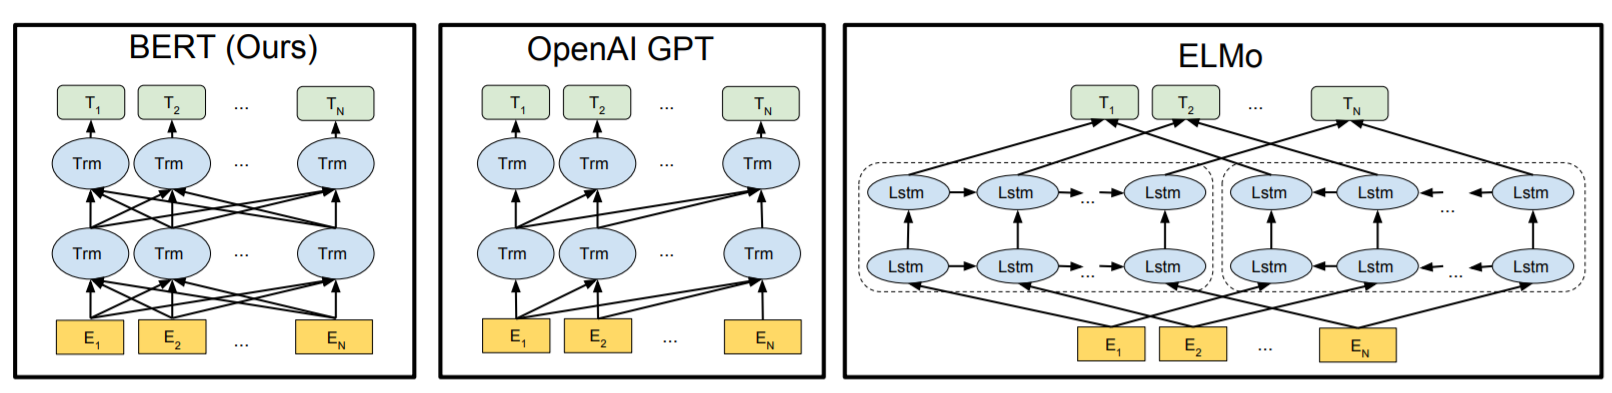
\includegraphics[width=0.9\textwidth]{imgs/bert_vs_elmo_vs_gpt.png}
\vspace{-5pt}
\caption{\footnotesize Comparing pre-training models: BERT uses a \hyperref[sec:BidirectionalLM]{bidirectional} \nameref{sec:Transformer}. OpenAI GPT uses a \hyperref[sec:ForwardLM]{forward} \nameref{sec:Transformer}. \nameref{sec:ELMo} combines independently-trained \hyperref[sec:ForwardLM]{forward} and \hyperref[sec:BackwardLM]{backward} \hyperref[sec:LSTM]{LSTM}s. Among the three, only BERT embeddings are jointly conditioned on forward and backward context in all layers. Alongside architectural differences, BERT and OpenAI GPT are fine-tuning approaches, while ELMo is a feature-based approach (Devlin et al., 2019). \textit{NOTE: $E_n =$ the $n$-th token in the input sequence, and $T_n =$ the corresponding output embedding}. From \emph{BERT: Pre-training of Deep Bidirectional Transformers for Language Understanding}, by Devlin et al., 2019. \url{https://arxiv.org/pdf/1810.04805.pdf}. Copyright 2019 by Devlin et al.}
\vspace{-5pt}
\label{fig:NAME}
\end{figure}





\subsection{Motivation for BERT} \label{sec:MotivationForBERT}

Instead of using \nameref{sec:ELMo}'s ``shallow" combination of ``independently-trained" \hyperref[sec:BidirectionalLM]{biLM}s, ``BERT is designed to pre-train deep bidirectional representations from unlabeled text by jointly conditioning on \emph{both} left and right context in all layers" (Devlin et al., 2019). \textbf{BERT (Bidirectional Encoder Representations from Transformers)} combines a \hyperref[sec:BidirectionalLM]{biLM}, \hyperref[sec:SelfAttention]{self attention}, and \nameref{sec:Transformer} (more powerful than \hyperref[sec:LSTM]{LSTM}s), and also a \hyperref[sec:maskedlanguagemodelMLM]{masked language model (MLM)}, yielding vast performance gains over previous models (Wiedemann et al., 2019).   


%Another motivation for BERT stems from previous limitations. The \textbf{OpenAI GPT} model uses a left-to-right construction, where each token only attends to past tokens in the \hyperref[sec:SelfAttention]{self attention} layers of the \nameref{sec:Transformer}. This approach performs poorly on \emph{sentence-level} and \emph{token-level} tasks, like \nameref{nlptask:questionansweringQA}, where \textbf{bidirectional context} is required.  






\subsection{Describing BERT} \label{sec:DescribingBERT}

\subsubsection{Input Embedding in BERT} \label{sec:BERTInputEmbedding}

The input embedding in BERT is created by summing three kinds of embeddings: 

\begin{enumerateSpaced}{3pt}
    \vspace{-10pt}
    \item \textbf{\textit{WordPiece} token embeddings: }The \emph{WordPiece} \nameref{nlptask:tokenization} strategy, instead of tokenizing by the natural separations between English words, subdivides words into smaller, basic units. For example, the WordPiece \nameref{nlptask:tokenization} of ``playing" might be ``play" + ``**ing". This allows BERT to handle rare, unknown words (Weng, 2019) and reduce vocabulary size while increasing amount of data available per word. For instance, if ``play" and ``**ing" and ``**ed" are present in the vocabulary but ``playing" and ``played" are not, then these can be recognized by their sub-units. 
    
    \item \textbf{Segment embeddings: }are  arbitrary spans of contiguous text made by packing sentence parts together. Contrary to BERT,  \nameref{sec:TransformerXL}'s \textbf{segment embeddings} respect sentence boundaries. 
    
    \item \textbf{\hyperref[sec:PosEncodings]{Positional embeddings}: } same as in the \nameref{sec:Transformer}, to account for word ordering. 
\end{enumerateSpaced}


\subsubsection{BERT's Framework}
 
There are two steps in BERT's framework: \textbf{pre-training}, in which BERT trains on \emph{unlabeled data} over different tasks, and \textbf{fine-tuning}, in which BERT is initialized with the pre-training parameters to train over \emph{labeled data} for specific \hyperref[app:Appendix_NLPTasks]{nlp tasks}. Pre-training using the \nameref{sec:maskedlanguagemodelMLM} and \nameref{sec:nextsentencepredictionNSP} tasks allows BERT to learn \textbf{bidirectional context} and \emph{sentence-level} information, as opposed to simple \hyperref[sec:LanguageModels]{language models} that predict subsequent tokens given context. 


\subsubsection{Masked Language Model (MLM)} \label{sec:maskedlanguagemodelMLM}

It is a well-known problem that bidirectional conditioning causes lower layers to leak information about tokens, so each word can implicitly ``see itself" letting the model trivially guess the target word in a multi-layered context (Devlin et al., 2019).  

BERT's solution is to use a \textbf{masked language model (MLM)}, which randomly masks some input tokens to predict original tokens using only context. This fuses left and right context to get \emph{deep} bidirectional context, unlike \nameref{sec:ELMo}'s shallow left-to-right language model (Devlin et al., 2019). However, the issue with masking is that it hampers BERT's performance. BERT only predicts the \texttt{[MASK]} token when it is present in the input, even though BERT should predict correct tokens regardless of which tokens are present in input (Kurita, 2019a). As a solution, BERT varies its masking strategy: (1) replace the word to be masked with \texttt{[MASK]} only with $80\%$ probability; (2) replace the word to be masked with a random word $10 \%$ of the time; and (3) keep the masked word $10 \%$ of the time. 


\subsubsection{Next Sentence Prediction (NSP)} \label{sec:nextsentencepredictionNSP}

Ordinary \hyperref[sec:LanguageModels]{language models} perform badly for tasks requiring sentence-level knowledge, like \nameref{nlptask:questionansweringQA} and \nameref{nlptask:naturallanguageinferenceNLI}. Thus, BERT pre-trains on a \textbf{next sentence prediction (NSP)} task to practice determining if one sentence is the next sentence of the other. 

%Training BERT using NSP is as follows: (1) sample sentence pairs \texttt{(A, B)} so that half the time \texttt{B} follows \texttt{A} (labeled as \texttt{IsNext}) and half the other time, \texttt{B} does not follow \texttt{A} (labeled as \texttt{NotNext}), then (2) BERT processes both sentences and uses a binary classifier to decide of \texttt{B} is the next sentence after \texttt{A} (Weng, 2019). 


\subsection{Experimental Results of BERT} \label{sec:BERTExperimentalResults}


% NOTE: the top width must be +0.5 more than below texwidth measure
%\begin{program}
% 
{
\begin{wrapfigure}{L}{0.45\textwidth}
    \begin{center}
    \vspace{-30pt}
    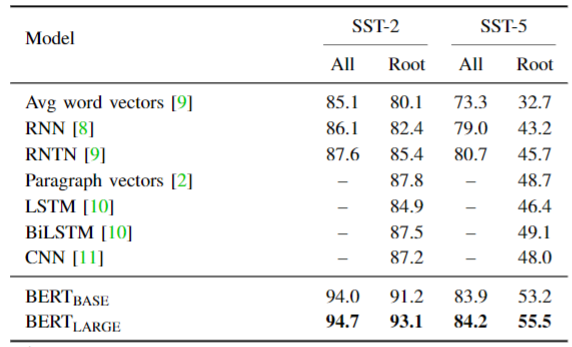
\includegraphics[width=\linewidth]{imgs/table_bertExperimentalResults.png}
    \end{center}
\vspace{-15pt}
\captionof{table}{Accuracy (\%) of several models on \nameref{nlptask:sentimentclassificationSC} SST dataset. BERT has highest accuracy scores. From \emph{Table B.II in Fine-Grained Sentiment Classification Using BERT}, by Munikar et al., 2019. \url{https://arxiv.org/pdf/1910.03474.pdf}. Copyright 2019 by Munikar et al.}
%\vspace{30pt}
\label{tbl:bertExperimentResults}
\end{wrapfigure}

Using a simple accuracy measure, Munikar et al. (2019) found that a pre-trained BERT model fine-tuned for \nameref{nlptask:sentimentanalysisSA} task outperformed complex models such as \hyperref[sec:RNN]{RNN}s and CNNs. The \cref{tbl:bertExperimentResults} includes results on phrases and entire reviews. 

This proves \nameref{nlptask:transferlearning} is possible with BERT's deep contextual \hyperref[sec:BidirectionalLM]{bidirectional language model}.





\subsection{Probing BERT} \label{sec:ProbingBERT}

BERT has surpassed state-of-the-art performance in a wide range of \hyperref[app:Appendix_NLPTasks]{nlp tasks} but it is not known why. Clark et al. (2019) use an ``attention-based probing classifier" to study BERT's internal vector representations to understand what kinds of linguistic features BERT learns from its self-supervised training on unlabeled data. 


%\end{program}


\subsubsection{BERT Learns Dependency Syntax} \label{sec:BERTLearnsSyntax}

Firstly, Clark et al. (2019) found that BERT's attention heads behave similarly, like focusing on positional offsets or attending broadly over an entire sentence. 

}


Secondly, while individual attention heads do not capture syntax dependency structure as a whole, certain heads are better at detecting various syntax dependency relations. For example, the heads detect ``direct objects of verbs, determiners of nouns, objects of prepositions, and objects of possessive pronouns with > $75 \%$ accuracy (Clark et al., 2019). 



\begin{figure}
\centering
\begin{minipage}{.35\textwidth}
  \centering
  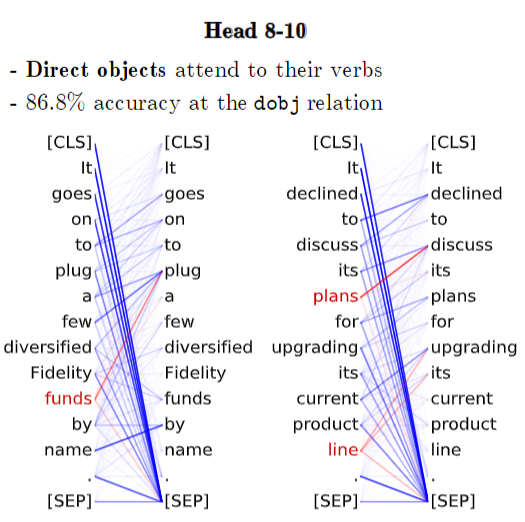
\includegraphics[width=\textwidth]{imgs/bert_headsDirectObject.png}
  \captionof{figure}{\scriptsize In heads 8-10, direct objects attend to their verbs. Line darkness indicates attention strength. Red indicates attention to/from red words, to highlight certain attentional behaviors. From \emph{What Does BERT Look At? An Analysis of BERT's Attention}, by Clark et al., 2019. \url{https://arxiv.org/abs/1906.04341}. Copyright 2019 by Clark et al.}
  \label{fig:bertHeadDirectObject}
\end{minipage} \hspace{2em}%
\begin{minipage}{.35\textwidth}
  \centering
  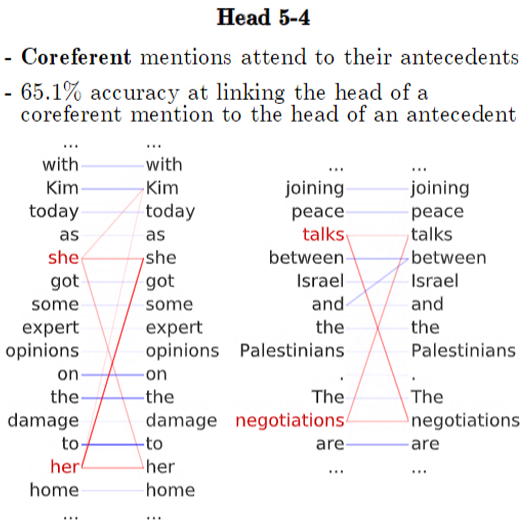
\includegraphics[width=\textwidth]{imgs/bert_headsCoref.png}
  \captionof{figure}{\scriptsize In heads 5-4, BERT does \nameref{nlptask:coreferenceresolutionCR} by linking the head of a coreferent mention to the head of an antecedent. From \emph{What Does BERT Look At? An Analysis of BERT's Attention}, by Clark et al., 2019. \url{https://arxiv.org/abs/1906.04341}. Copyright 2019 by Clark et al.}
  \vspace{-10pt}
  \label{fig:bertCoref}
\end{minipage}
\end{figure}


Attention heads 8-10 in \cref{fig:bertHeadDirectObject} learn how direct objects attend to their verbs, and achieves high accuracy at the direct object relation task. The fact that BERT learns this via self-supervision coupled with the heads' propensity for learning syntax may explain BERT's success. Attention heads 5-4 in \cref{fig:bertCoref} perform \nameref{nlptask:coreferenceresolutionCR}. This task is more challenging than syntax tasks since \hyperref[nlptask:coreferenceresolutionCR]{coreference} links span longer than syntax dependencies, and even state-of-the-art models struggle at this task.



\subsubsection{BERT's Contribution In Polysemy and Word Sense Disambiguation} % PAPER: DOEs bert make any sense


Using a kNN classification, Wiedemann et al. (2019) compared the \hyperref[sec:SolutionWithContextEmbs]{contextual embedding}s of \nameref{sec:ELMo} and BERT on \nameref{nlptask:wordsensedisambiguatioNWSD} and found BERT places \hyperref[sec:Polysemy]{polysemic} words into distinct regions according to their senses, while \nameref{sec:ELMo} cannot since word senses in ELMo's embedding space are less sharply clustered.

Further, in \cref{tbl:bertPolysemy} Wiedemann et al. (2019) study how BERT matched word senses from the test set to given \hyperref[sec:Polysemy]{polysemic} word from a training set. BERT predicted correctly when the text had \emph{vocabulary overlap} like in example (2) ``along the \emph{bank} of the river" (the input text) and ``along the \emph{bank} of the river Greta" (nearest neighbor found by BERT). BERT also predicted correctly when text had \emph{semantic overlap}, like in example (3) ``little earthy bank" (input) ``huge bank [of snow]" (nearest neighbor found by BERT). 


However, BERT struggled when facing \emph{vocabulary and semantic overlap in conjunction}. Example (5) in \cref{tbl:bertPolysemy} shows BERT predicted ``land bank" as in a \emph{supply or stock} but the correct sense of ``land bank" was \emph{financial institution}. Distinguishing verb senses was trickier: in example (12), the correct sense label of \hyperref[sec:Polysemy]{polysemic} ``watch" was \emph{to look attentively} while BERT predicted its sense as \emph{to follow with the eyes or the mind; observe}. 

%Despite BERT's limitations, the authors conclude still that BERT captures \hyperref[sec:Polysemy]{polysemy} more successfully than \nameref{sec:ELMo}, inspiring future work for using \nameref{nlptask:wordsensedisambiguatioNWSD} to compare BERT to models like \nameref{sec:XLNet}. 


\begin{figure}[h]
\vspace{-5pt}
\centering
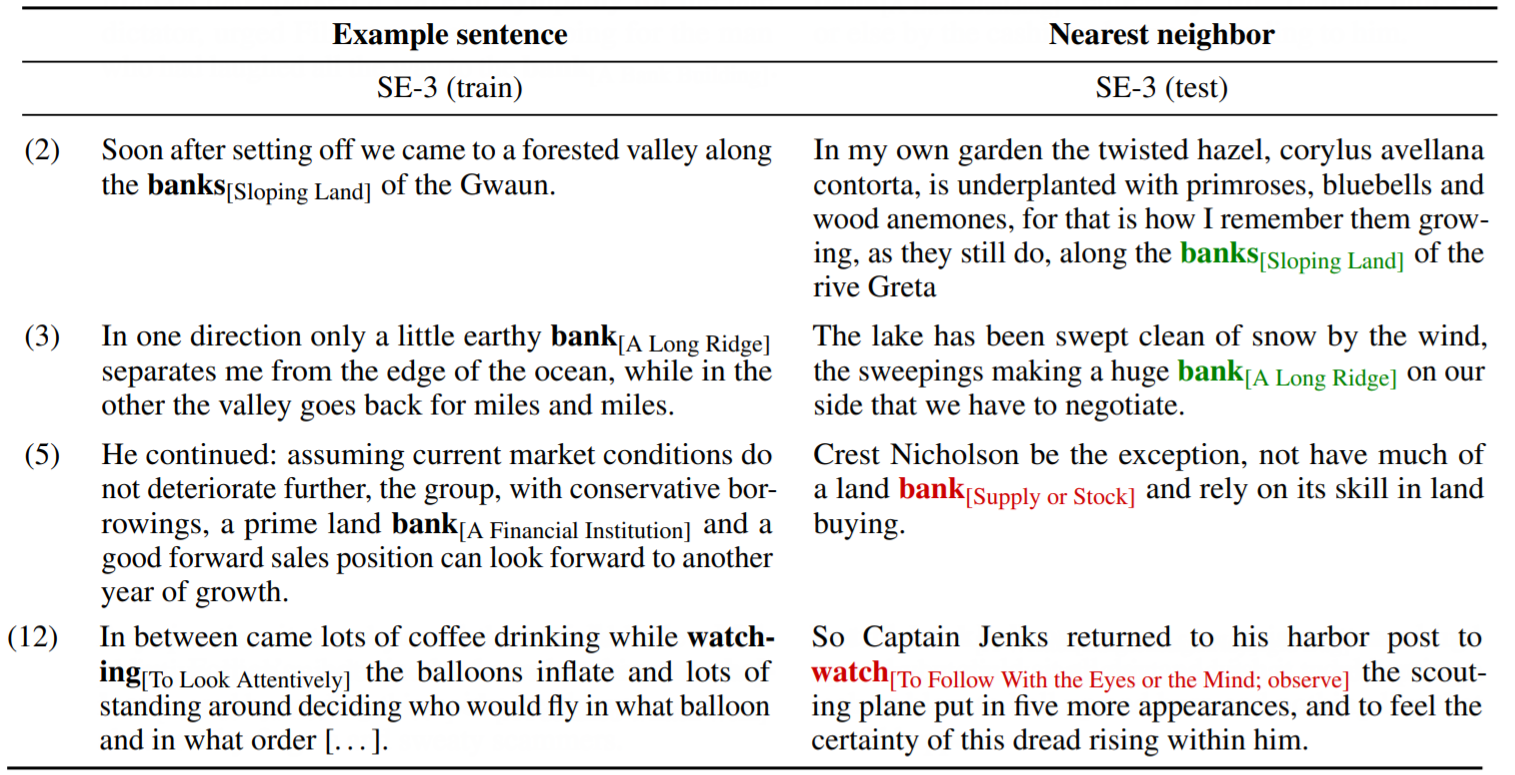
\includegraphics[width=0.85\textwidth]{imgs/table_bertPolysemyComparisons.png}
\vspace{-5pt}
\captionof{table}{Example predictions by BERT based on nearest neighbor sentences. The \hyperref[sec:Polysemy]{polysemic} word is \textbf{bolded}, and has a WordNet description tag describing its correct sense to be predicted. \textbf{True positives by BERT are {\color{ForestGreen} green}} while \textbf{false positives made by BERT are {\color{FireBrick}red}}. From (adapted) Table 4 in \emph{Does BERT Make Any Sense? Interpretable Word Sense Disambiguation with Contextualized Embeddings}, by Wiedemann et al., 2019. \url{https://arxiv.org/pdf/1909.10430.pdf}. Copyright 2019 by Wiedemann et al.}
\label{tbl:bertPolysemy}
\vspace{-5pt}
\end{figure}